\section{Date: 2026-09-19}
\noindent \textbf{Series ID: JTU6200OSR} 

\noindent This series is titled Other Separations: Health Care and Social Assistance and has a frequency of Monthly. The units are Rate and the seasonal adjustment is Not Seasonally Adjusted.The observation start date is 2000-12-01 and the observation end date is 2026-07-01.The popularity of this series is 1. \\ 

\noindent \textbf{Series ID: JTU4400HIR} 

\noindent This series is titled Hires: Retail Trade and has a frequency of Monthly. The units are Rate and the seasonal adjustment is Not Seasonally Adjusted.The observation start date is 2000-12-01 and the observation end date is 2026-07-01.The popularity of this series is 1. \\ 

\subsection{Raw Regression}
\noindent Regresses the two series against each other directly. A significant result here can come just as easily from both series sharing a long-run trend as from any real relationship.

\begin{center}
\begin{tabular}{lclc}
\toprule
\textbf{Dep. Variable:}          & value\_fred\_JTU4400HIR & \textbf{  R-squared:         } &     0.011   \\
\textbf{Model:}                  &           OLS           & \textbf{  Adj. R-squared:    } &     0.007   \\
\textbf{Method:}                 &      Least Squares      & \textbf{  F-statistic:       } &     3.313   \\
\textbf{Date:}                   &     Sat, 19 Sep 2026    & \textbf{  Prob (F-statistic):} &   0.0697    \\
\textbf{Time:}                   &         14:54:03        & \textbf{  Log-Likelihood:    } &   -414.91   \\
\textbf{No. Observations:}       &             308         & \textbf{  AIC:               } &     833.8   \\
\textbf{Df Residuals:}           &             306         & \textbf{  BIC:               } &     841.3   \\
\textbf{Df Model:}               &               1         & \textbf{                     } &             \\
\textbf{Covariance Type:}        &        nonrobust        & \textbf{                     } &             \\
\bottomrule
\end{tabular}
\begin{tabular}{lcccccc}
                                 & \textbf{coef} & \textbf{std err} & \textbf{t} & \textbf{P$> |$t$|$} & \textbf{[0.025} & \textbf{0.975]}  \\
\midrule
\textbf{const}                   &       4.9928  &        0.175     &    28.499  &         0.000        &        4.648    &        5.338     \\
\textbf{value\_fred\_JTU6200OSR} &      -1.5143  &        0.832     &    -1.820  &         0.070        &       -3.151    &        0.123     \\
\bottomrule
\end{tabular}
\begin{tabular}{lclc}
\textbf{Omnibus:}       &  5.215 & \textbf{  Durbin-Watson:     } &    0.754  \\
\textbf{Prob(Omnibus):} &  0.074 & \textbf{  Jarque-Bera (JB):  } &    5.214  \\
\textbf{Skew:}          &  0.318 & \textbf{  Prob(JB):          } &   0.0737  \\
\textbf{Kurtosis:}      &  2.971 & \textbf{  Cond. No.          } &     16.3  \\
\bottomrule
\end{tabular}
%\caption{OLS Regression Results}
\end{center}

Notes: \newline
 [1] Standard Errors assume that the covariance matrix of the errors is correctly specified.

\begin{figure}
\centering
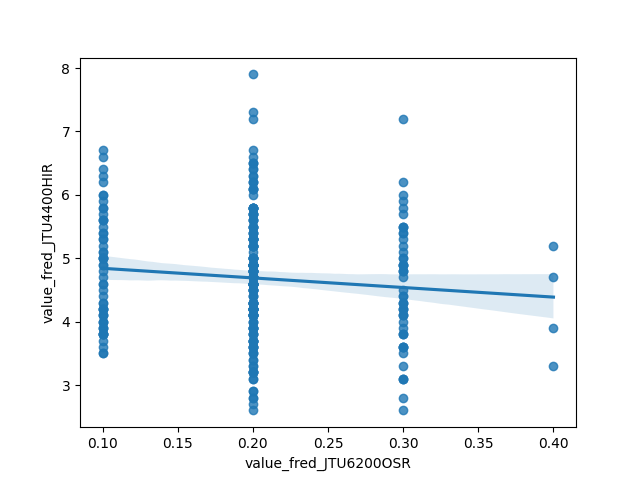
\includegraphics[scale = 0.9]{plots/plot_2026-09-19.png}
\caption{Raw Regression Plot for 2026-09-19}
\end{figure}
\newpage
\subsection{Detrended Regression}
\noindent Regresses the residuals of each series after removing its own linear time trend, so a shared trend can no longer drive the result on its own. A relationship that stays significant here is better evidence of a genuine link between the two series.

\begin{center}
\begin{tabular}{lclc}
\toprule
\textbf{Dep. Variable:}                     & value\_fred\_JTU4400HIR\_detrended & \textbf{  R-squared:         } &     0.023   \\
\textbf{Model:}                             &                OLS                 & \textbf{  Adj. R-squared:    } &     0.020   \\
\textbf{Method:}                            &           Least Squares            & \textbf{  F-statistic:       } &     7.277   \\
\textbf{Date:}                              &          Sat, 19 Sep 2026          & \textbf{  Prob (F-statistic):} &  0.00737    \\
\textbf{Time:}                              &              14:54:03              & \textbf{  Log-Likelihood:    } &   -409.05   \\
\textbf{No. Observations:}                  &                  308               & \textbf{  AIC:               } &     822.1   \\
\textbf{Df Residuals:}                      &                  306               & \textbf{  BIC:               } &     829.6   \\
\textbf{Df Model:}                          &                    1               & \textbf{                     } &             \\
\textbf{Covariance Type:}                   &             nonrobust              & \textbf{                     } &             \\
\bottomrule
\end{tabular}
\begin{tabular}{lcccccc}
                                            & \textbf{coef} & \textbf{std err} & \textbf{t} & \textbf{P$> |$t$|$} & \textbf{[0.025} & \textbf{0.975]}  \\
\midrule
\textbf{const}                              &     7.77e-13  &        0.052     &  1.49e-11  &         1.000        &       -0.103    &        0.103     \\
\textbf{value\_fred\_JTU6200OSR\_detrended} &      -2.2825  &        0.846     &    -2.698  &         0.007        &       -3.947    &       -0.618     \\
\bottomrule
\end{tabular}
\begin{tabular}{lclc}
\textbf{Omnibus:}       &  7.615 & \textbf{  Durbin-Watson:     } &    0.790  \\
\textbf{Prob(Omnibus):} &  0.022 & \textbf{  Jarque-Bera (JB):  } &    7.440  \\
\textbf{Skew:}          &  0.352 & \textbf{  Prob(JB):          } &   0.0242  \\
\textbf{Kurtosis:}      &  3.289 & \textbf{  Cond. No.          } &     16.2  \\
\bottomrule
\end{tabular}
%\caption{OLS Regression Results}
\end{center}

Notes: \newline
 [1] Standard Errors assume that the covariance matrix of the errors is correctly specified.

\begin{figure}
\centering
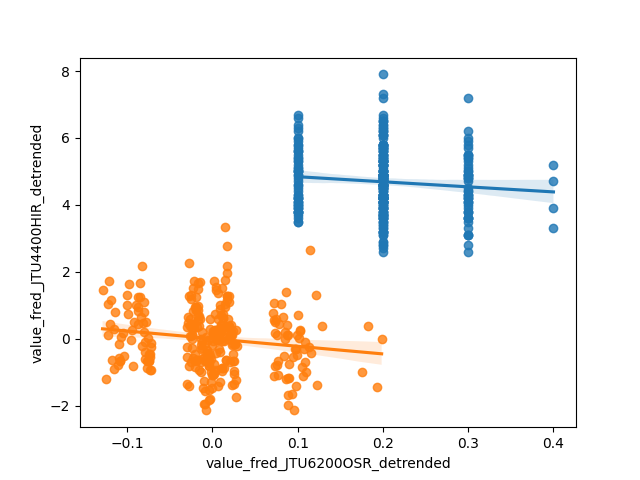
\includegraphics[scale = 0.9]{plots/plot_2026-09-19_detrended.png}
\caption{Detrended Regression Plot for 2026-09-19}
\end{figure}
\newpage
